\section{Proposed solution}\label{solution}

In a typical microservices application, who is communicating is less important than the data being exchanged. To give priority to the data rather than to hosts, we will design an Information-centric network ~\cite{Ahlgren} between microservices using NDN network stack ~\cite{zhang2014named}. This new network design will facilitate two important services that can help microservices to exchange and cache REST objects efficiently without using any additional middleware. Two important goals of our new network.

\subsection{Main features of new network}
 \begin{enumerate}
     \item \textbf{Service discovery}
      \begin{enumerate}
          \item Each REST service endpoint will have a unique global name in an application namespace.
            \item Every microservice inside an application namespace will have the capability to request objects of data from any other endpoint inside the same namespace.
            \item The network will have a capability to propagate requested objects through the network to the requester.
     \end{enumerate}
 
 \item \textbf{In-network cache}
   \begin{enumerate}
    \item We will provide a capability for in-network storage ~\cite{zhang2014named} of objects which can decrease latency and improve the reliability of the application. 
   \end{enumerate}
 \end{enumerate}
 
 To achieve above-said goals, we will describe the architecture of the new network model in next section.
 \subsection{Implementation}
\subsubsection{Overview of design }

To transfer REST protocol objects efficiently on an NDN network, we need to develop a client library that can be attached to a microservice and helps in setting up connection, transferring of REST objects through NDN forwarder and closing of the NDN connection. We need a content store with REST specific caching policy so that we can take advantage of cacheable REST objects.

As part of our project, our main contributions will be

\begin{enumerate}
\item REST - NDN client library for python based microservice.
\item Design and implementation of a content store for REST objects.
\item Evaluate the performance of the REST protocol with NDN as transport.
\end{enumerate}

\subsubsection{REST - NDN client library}

We will develop a REST-NDN client library in python which will give a capability of taking REST commands from application code through an API and sending NDN objects into the network. This library will also help clients to specify cache specific parameters like freshness which will be used by the content store. Each microservice will have a client library which will help in connecting to the NDN forwarding demon. Each physical node will have an NDN forwarding demon capable of routing NDN packets through the network (see figure  ~\ref{fig:networkmodel}).

\subsubsection{Addressing schema}

In our addressing scheme, each REST endpoint is addressable. Every REST endpoint will have a globally unique name. 

\begin{center} \url{ Endpoint/instance_count/version  } \end{center}
\begin{center} Naming structure of a endpoint  \end{center}

This addressing schema is simple enough but serves to achieve the required features.
\begin{enumerate}
\item By using only unique REST endpoint name and removing references to a microservice name, we can decouple endpoints from hosting microservices. This will help to decrease downtime and unnecessary changes when endpoints are moved between services.
\item  Having an instance count can help identify and load balance among different instances of the same REST endpoint.
\item version helps in maintaining two versions of same endpoint available at the same time. This can facilitate rolling updates.  
\end{enumerate}


\subsubsection{Connecting new microservice to the network}

Newly created microservice using our REST-NDN client will broadcast in its own local container bridge ~\cite{DockerNet} for local NDN forwarder IP address. Once it receives IP address it will use Named Data Link State Routing Protocol ~\cite{hoque2013nlsr} to advertise all its objects to the local router. We will configure our NDN forwarder to only advertise longest common name for all other forwarders. In this way, we can have few updates while maintaining load balance between distributed endpoints.

\begin{figure}
   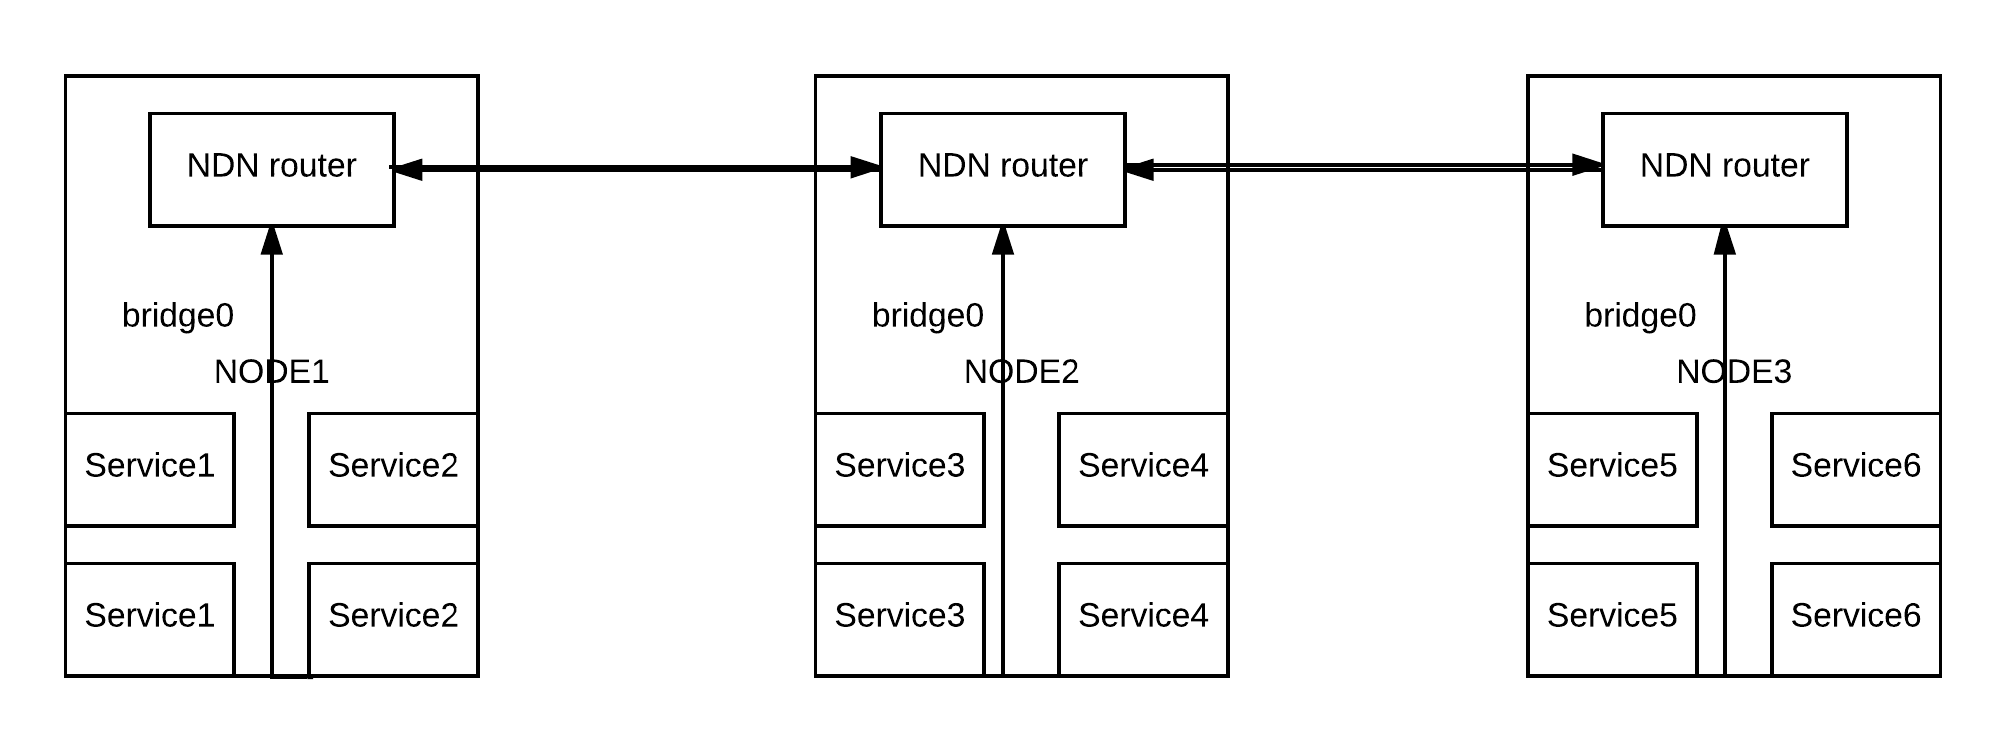
\includegraphics[height=3cm, width=8cm]{figs/structural_diagram}
   \caption{Architecture of proposed network.}
   \label{fig:networkmodel}
\end{figure}

\subsubsection{Content store}

We will design a caching system which will be attached to NDN forwarder. This caching system will have the capability to understand REST specific cache parameters set by REST-NDN clients. This cache will also improve the reliability microservices application by returning the most updated value of the REST object in case of network failure.

\subsubsection{Named routing}

There will be an NDN forwarding demon ~\cite{NFD} ~\cite{zhang2014named} in every physical node (see Fig. ~\ref{fig:networkmodel}). This forwarder will be connected to all other containers in the same node using a bridge~\cite{DockerNet}. We will replace default content store for REST specific content store.
NDN uses NLSR - Named Data Link State Routing Protocol ~\cite{hoque2013nlsr} to transfer new REST endpoint information among router overlay network.


